% !TEX root = ../notes_template.tex
\chapter{Demand Systems}\label{chp:Demand_Systems}

%\minitoc

%gls examples:
%\begin{itemize}
%	% \item \glsxtrshort{gcd};
%	\item \Gls{gcd}; \acrlong{gcd}; \acrshort{gcd}; \acrfull{gcd}
%\end{itemize}


\paragraph{}{The use of demand systems dates back to the early 20th century. }

\paragraph{Three conditions on demand systems in theoretical work\\}{
	\begin{itemize}
		\item Additivity\\
		Sum of the expenditures given by the system equals to total expenditure. 
			\begin{equation}\label{eq2.0.1a}
				p'q \equiv \mu.
			\end{equation}
		
		\item Homogeneity\\
		Sum of the expenditures given by the system equals to total expenditure. 
			\begin{equation}\label{eq2.0.1b}
				\hat{q}^{-1}(a \mu + Ap) \equiv 0.
			\end{equation}
	
		\item Symmetry of the substitution matrix\\
		Sum of the expenditures given by the system equals to total expenditure. 
			\begin{equation}\label{eq2.0.1c}
				S \equiv S',
			\end{equation}
		or we can write it as $s_{i,j}=s_{j,i}$, where the substitution matrix $S$ is defined
			\begin{equation}\label{eq2.0.1d}
				S=\hat{q}^{-1}(ai' + A\hat{q}^{-1})\mu
			\end{equation}
		
	\end{itemize}
}

%---- Section 2.1 ----%
%		  LES  		  %
%%%%%%%%%%%%%%%%%%%%%%%
\section{Linear Expenditure System (LES)}
\cite{Stone1954}
\paragraph{}{Linear expenditure system, first described by \cite{Stone1954}, laid the foundation of the development of other flexible demand systems, like the Quadratic Expenditure System (QES), the Almost Ideal Demand System (AUDS), the Quadratic Almost Ideal Demand System (QUAIDS), An Implicitly Directly Additive Demand System (AIDADS), etc. The core idea of LES, and its implementation, is summarized in the following sections. }

\subsection{The theoretic framework of  LES}
\paragraph{}{Expenditures on individual commodities are expressed as linear functions of total expenditure $\mu$ and price $p_i$.
	\begin{equation}\label{eq2.1.1}
		\hat{p}q = \hat{p} \bar{q} + b(\mu - p' \bar{q}),
	\end{equation}
where $p$ is a price vector, $q$ is a quantity vector, $\bar{q}$ is a quantity vector to which consumers are committed (subsistent level of consumption), $b$ is a constant proportion vector indicating a certain proportion of supernumerary income, $\sum_{i=1}^{m}b_i=1$. Consumers first use up $\hat{p}\bar{q}$ of the income for certain goods and then distribute the remaining income over a  set of available commodities in fixed proportion, indicated by $b$. \\

Therefore, $\hat{p}q$ gives the expenditures on the commodities (the $i_{th}$ diagonal element is the expenditure on the $i_{th}$ commodity), $\hat{p}\bar{q}$ is the basic (subsistent) consumption of commodities. $p'\bar{q}$ is the total committed expenditure (to the subsistent consumption), $(\mu - p' \bar{q})$ is the supernumerary income.\\

It could be broken down into \cref{eq2.1.2} and \cref{eq2.1.3}.
	\begin{equation} \label{eq2.1.2}
		\hat{p}q = b \mu + Bp,
	\end{equation}

	\begin{equation} \label{eq2.1.3}
		B = (bi'-I)\hat{c},
	\end{equation}
where $i$ is a unit vector, $I$ is a unit matrix, and $-\hat{c} = -q$. 
}


\section{Quadratic Expenditure System(QES)}
%---- 1.1.1 Subsection 1 ----%
\subsection{The theoretic framework of QES}
\paragraph{}{QES exploits the full potential of Engel curve flexibility and can be estimated with a relatively small number of free parameters. }

\paragraph{Indirect Utility Function}{Each theoretically plausible quadratic expenditure system is generated by the indirect utility function \cref{eq2.2.1}
	\begin{equation}\label{eq2.2.1}
		\Psi(P,\mu) = -\frac{g(P)}{\mu - f(P)} - \frac{\alpha (P)}{g(P)},
	\end{equation}
where $P^T=(p_1 p_2 ... p_n)$ is the vector of prices for $n$ commodity groups and $\mu$ denotes total expenditure. 
}

\paragraph{Demand Functions Quadratic in Expenditure\\}{
\cite{Howe1979} defined a system of demand functions quadratic in expenditure, by the indirect utility function, of the form
	\begin{equation} \label{eq2.2.2}
		h_i(P,\mu) = \frac{1}{g^2}(\partial \alpha - \frac{\partial g}{g} \alpha) \mu^2 + [\frac{\partial g}{g} - \frac{2f}{g^2}(\partial \alpha -\frac{\partial g}{g} \alpha )] \mu + \frac{f^2}{g^2}(\partial \alpha - \frac{\partial g}{g} \alpha) - \frac{\partial g}{g}f + \partial f,
	\end{equation}
where $f$, $g$, and $\alpha$ are functions homogeneous of degree one, equivalently
	\begin{equation} \label{eq2.2.3}
		h_i(P,\mu) = \frac{1}{g^2}(\partial \alpha - \frac{\partial g}{g} \alpha) (\mu - f)^2 + \frac{\partial g}{g} (\mu - f) + \partial f.
	\end{equation}

 \small{A \textit{homogeneous function} is a function of several variables such that, if all its arguments are multiplied by a scalar, then its value is multiplied by some power of this scalar, called \textit{the degree of homogeneity}, or simply the degree; that is, if k is an integer, a function f of n variables is homogeneous of degree k if
	\begin{equation}\label{eq2.3a}
		f(sx_1,...,sx_n)=s^kf(x_1,...,x_n)  
	\end{equation}
for every $x_1,..,x_n$, and $s \neq 0$.
 }
}

\paragraph{The system for implementation\\}{
	The system easy for implementation is characterized by the indirect utility function \cref{eq2.2.4.1} 
	\begin{equation}\label{eq2.2.4.1}
		\Psi(P,\mu) = -\frac{\prod_i^n P_i^{a_i}}{\mu - \sum_{i}^{n} p_i {\widehat b}_i} - \frac{\sum_{i}^{n} p_i c_i}{\prod_{i}^{n}p_i^{a_i}},
	\end{equation}
	and the expenditure functions \cref{eq2.2.4.2}
	\begin{equation}\label{eq2.2.4.2}
		p_i q_i(P,\mu) = p_i \widehat{b}_i + a_i (\mu - \sum_{j} p_j \widehat{b}_j) + (c_i p_i - \sum_{j} p_j c_j) \prod_{j} p_j^{2a_j}(\mu - \sum_j p_j \widehat{b}_i)^2.
	\end{equation}	
	under the following constraints.
	\begin{equation}\label{eq2.2.4a}
		g(P) = \prod_{i}^{n}p_i^{a_i}
	\end{equation}

	\begin{equation}\label{eq2.2.4b}
		f(P) = \sum_{i}^{n} p_i \widehat{b}_i
	\end{equation}

	\begin{equation}\label{eq2.2.4c}
		\alpha (P)= \sum_{i}^{n} p_i c_i
	\end{equation}

	\begin{equation}\label{eq2.2.4d}
		\sum_{i}^{n} a_i = 1
	\end{equation}

	The system has $3n-1$ free parameters, for each of the commodity exists a parameter set \{$a_i$, $\widehat{b}_i$, $c_i$\}.
 }




%---- 2.1.2 Section 1.2 ----%
\subsection{Examples}
\paragraph{Estimation in Germany\\}{\cite{SCHULTE2017512}\\}

\paragraph{}{This paper applied a quadratic expenditure system to project the \textbf{cross- and own- price elasticiteis} and \textbf{income- (expenditure) elasticities of residential energy demand (heating and electricity)} in Germany using the official expenditure data from 1993 to 2008.}

\paragraph{Definition\\}{They distinguished 10 commodities, as shown in \cref{fig2.1}, and estimated their mean expenditure, own-price and cross-price elasticities \cref{fig2.2} at the national average level. Six household type (\cref{fig2.3}) and the income quartiles were distinguished to examine the income (expenditure) (\cref{fig2.4}) and price elasticities (\cref{fig2.5}) of energy demand in different households. }

\paragraph{Expenditure elasticity\\}{At the expenditure elasticities of electricity, heating increased with income level (ranging from 0.253 to 0.495 for electricity, from 0.279 to 0.452 for heating) and from single households to coupled households.  
}

\paragraph{Price elasticity\\}{At the national average level, the own-price elasticities of electricity, heating are -0.4310 and -0.5008, indicating a price-inelastic residential energy demand in Germany. Higher income households showed greater elasticity in both electricity and heating demand (around 3 times in the top quartile than in the bottom). Elasticity also grew from single households to coupled households.
}

\paragraph{Stone-Lewbel Cross Section Prices\\}{They reflect the fact that the composition of consumed commodity groups differs among households, making the perceived price of the commodity groups different among households. It is based on a theory of household specific price indices under the \textit{weakly separable} demand assumption.//
	In the case of Cobb-Douglas \textit{within group utility functions}, the price indices could be constructed as
	\begin{equation}\label{eq2.2.5a}
		u_i(q_i, s)=g_i \prod_h q_{ih}^{w_ih(s)},   \qquad \qquad \sum_{h}w_{ih} = 1,
	\end{equation}
where $i$ is the commodity group, $h$ is the composite in commodity group $i$, $s$ denotes a demographic characteristics vector, $g_i$ is the scaling factor for the commodity group, $q_{ih}$ is the consumed quantity and $w_{ih}$ is the (within group) budget share of good $h$ in group $i$. \\
	In this case, the household specific price index $p_i(s)$ is are derived as
	\begin{equation}\label{eq2.2.5b}
		p_i(s)=\frac{1}{g_i} \prod_{i} (\frac{\hat{p}_{ih}}{w_{ih}})^{w_{ih}},
	\end{equation}
whereby $\hat{p}_{ih}$ denotes prices for good $h$ of commodity group $i$ and the scaling factor $g_i$ represents



}


\begin{figure}[h]  % htbp
	\centering
	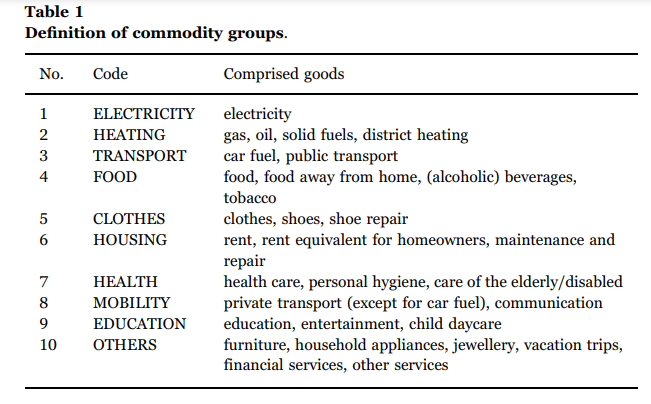
\includegraphics[width=0.8\textwidth]{./figure/ch2/fig2.1_table1.png}
	\caption{Commodity definition.}\label{fig2.1}
\end{figure}

\begin{figure}[h]  % htbp
	\centering
	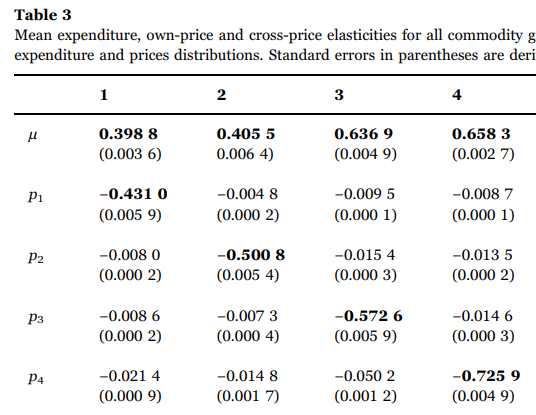
\includegraphics[width=0.8\textwidth]{./figure/ch2/fig2.2_table3.png}
	\caption{Mean expenditure, own-price and cross-price elasticities (electricity, heating, transport, food) at the national average level.}\label{fig2.2}
\end{figure}

\begin{figure}[h]  % htbp
	\centering
		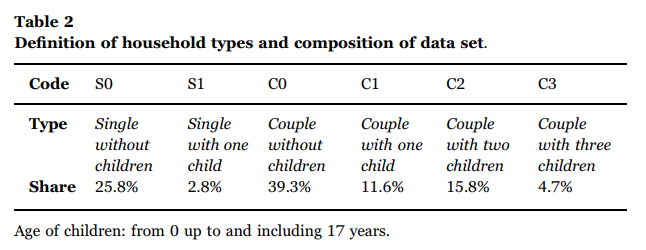
\includegraphics[width=0.8\textwidth]{./figure/ch2/fig2.3_table2.png}
	\caption{Household type.}\label{fig2.3}

\end{figure}

\begin{figure}[h]  % htbp
	\centering
	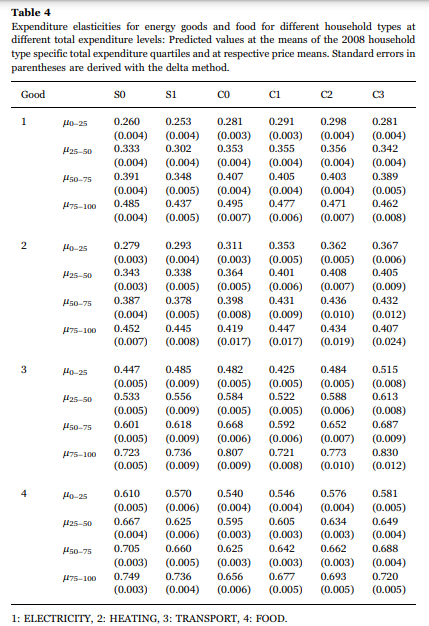
\includegraphics[width=0.8\textwidth]{./figure/ch2/fig2.4_table4.png}
	\caption{Income (expenditure) elasticities of electricity, heating, transport, and food demand in different households.}\label{fig2.4}
\end{figure}

\begin{figure}[h]  % htbp
	\centering
	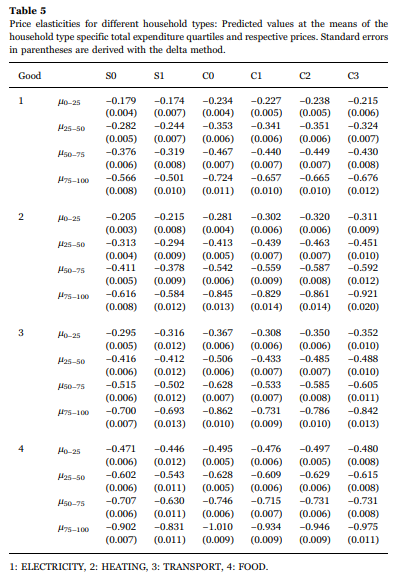
\includegraphics[width=0.8\textwidth]{./figure/ch2/fig2.5_table5.png}
	\caption{Price elasticities of electricity, heating, transport, and food demand in different households}\label{fig2.5}
\end{figure}


%---- Section 2.3 ----%
%\section{AIDADS}


% \end{minipage}
% \end{center}